Due to being electrically charged, electrons traversing the ID deposit energy until being ultimately absorbed in the ECal. Their trajectories can be reconstructed by combining ID tracks with energy deposits in the ECal. Particularly challenging for electron reconstruction is bremsstrahlung radiation which can occur due to detector material interactions. This process leads to two photon classifications:
\begin{itemize}
  \item \textbf{Converted photons}: Energy clusters in the ECal that are matched to a secondary vertex
  \item \textbf{Unconverted photons}: Energy clusters not matched to an electron track or a secondary vertex
\end{itemize}

Additional complications arises from other sources such as photons, hadronic jets, and non-prompt electrons that mimic genuine electrons but are not of physics interest. Figure~\ref{fig:reco_electron_track} illustrates an example path that an electron could take through the ATLAS detector.
%Should add citations where these can be read in more detail.
\begin{figure}[hpt]
  \centering
  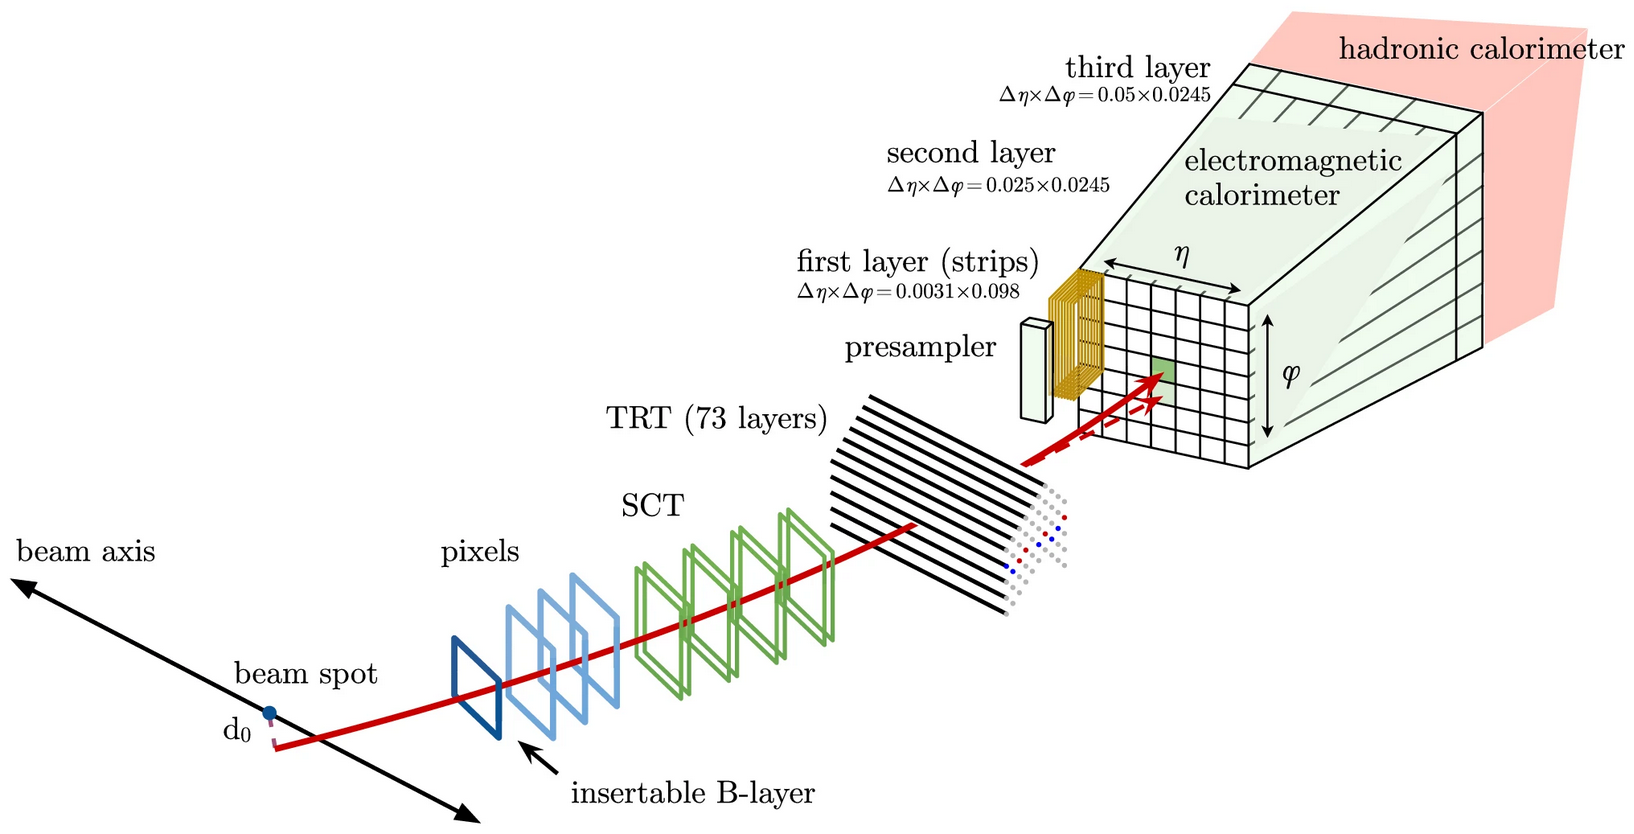
\includegraphics[width=0.65\textwidth]{figures/reco/reco_electron_track.png}
  \caption{Shown is an illustration of how an electron might travel through the ATLAS detector. As the electron passes through the TRT, bremsstrahlung radiation occurs, resulting in an electron and photon being absorbed in the ECal. The figure is taken from~\cite{ATLAS:2019jvq}.}\label{fig:reco_electron_track}
\end{figure}

The first step in the electron reconstruction chain is topo-cluster formation~\cite{ATLAS:2016krp}. These are constructed from proto-clusters in the ECal and HCal that have a calorimeter cell exceeding a predefined noise threshold. Neighboring cells that pass a lower threshold are then added and become seeds for the next iteration which continues until no seeds are left to try. If two proto-clusters have common cells, the clusters are merged. Proto-cluster containing two or more local maxima --- cells with at least 500 MeV deposited --- and four neighboring cells with lower energy deposits, are split into two clusters. Finally, these clusters are matched to ID tracks using the global $\chi^{2}$ fitter.

The next step in the reconstruction chain is the formation of superclusters that use topo-clusters as seed candidates. Superclusters are built by merging nearby satellite topo-cluster candidates that may have originated from bremsstrahlung or cluster splitting with the seed candidate provided selection criteria are satisfied. The supercluster formation algorithm proceeds as follows:
\begin{itemize}
  \item Clusters are sorted in descending order of $\et$
  \item Potential seed clusters are identified via:
  \begin{itemize}
    \item $\et > 1$ GeV
    \item A matched track with at least four hits in the silicon detectors
  \end{itemize}
  \item Reject clusters that are already satellites of another seed
\end{itemize}
Candidates that pass this are then used to find satellite clusters. A cluster is classified as a satellite if it is within $\Delta\eta \times \Delta\phi = 0.075 \times 0.125$ around the seed center, or within $\Delta\eta \times \Delta\phi = 0.125 \times 0.300$ and both clusters share the same best-matched tracks. The final supercluster is formed by merging the seed clusters with all associated satellite clusters.

During photon and electron reconstruction, superclusters are formed independently which can result in a cluster being identified as both an electron and photon candidate. These can be resolved by examining if the cluster is matched to a track vertex and whether a conversion vertex is present. If a cluster matches a track and no conversion vertex is found, it will likely be identified as an electron, and conversely if a conversion vertex is found without an associated track it will likely be a photon. 

In some cases, the classification remains ambiguous and could be either or photon or electron. These cases are left to the user allowing for classification decisions to be made based on the analysis needs.

Following electron reconstruction, an energy calibration and resolution step is applied to optimize energy resolution and correct the energy scale to have simulation match data. The calibration is performed with $Z\rightarrow e^{+}e^{-}$ events where scale factors are calculated in bins of $\eta$.

Electron reconstruction can be read in more detail in Ref~\cite{ATLAS:2019qmc} and~\cite{ATLAS:2019jvq}.
